\documentclass[aspectratio=169]{beamer}

%
% Choose how your presentation looks.
%
% For more themes, color themes and font themes, see:
% http://deic.uab.es/~iblanes/beamer_gallery/index_by_theme.html
%
\mode<presentation>
{
  \usetheme{default}      % or try Darmstadt, Madrid, Warsaw, ...
  \usecolortheme{default} % or try albatross, beaver, crane, ...
  \usefonttheme{default}  % or try serif, structurebold, ...
  \setbeamertemplate{navigation symbols}{}
  \setbeamertemplate{caption}[numbered]
  \setbeamertemplate{footline}[page number]
  \setbeamercolor{frametitle}{fg=white}
  \setbeamercolor{footline}{fg=black}
} 

\usepackage[english]{babel}
\usepackage[utf8x]{inputenc}
\usepackage{tikz}
\usepackage{listings}
\usepackage{courier}
\usepackage{bold-extra}
\usepackage{minted}
\usepackage{colortbl}

\xdefinecolor{darkblue}{rgb}{0.1,0.1,0.7}
\xdefinecolor{dianablue}{rgb}{0.18,0.24,0.31}
\definecolor{commentgreen}{rgb}{0,0.6,0}
\definecolor{stringmauve}{rgb}{0.58,0,0.82}

\lstset{ %
  backgroundcolor=\color{white},      % choose the background color
  basicstyle=\ttfamily\small,         % size of fonts used for the code
  breaklines=true,                    % automatic line breaking only at whitespace
  captionpos=b,                       % sets the caption-position to bottom
  commentstyle=\color{commentgreen},  % comment style
  escapeinside={\%*}{*)},             % if you want to add LaTeX within your code
  keywordstyle=\color{blue},          % keyword style
  stringstyle=\color{stringmauve},    % string literal style
  showstringspaces=false,
  showlines=true
}

\lstdefinelanguage{scala}{
  morekeywords={abstract,case,catch,class,def,%
    do,else,extends,false,final,finally,%
    for,if,implicit,import,match,mixin,%
    new,null,object,override,package,%
    private,protected,requires,return,sealed,%
    super,this,throw,trait,true,try,%
    type,val,var,while,with,yield},
  otherkeywords={=>,<-,<\%,<:,>:,\#,@},
  sensitive=true,
  morecomment=[l]{//},
  morecomment=[n]{/*}{*/},
  morestring=[b]",
  morestring=[b]',
  morestring=[b]"""
}

\title[2016-09-15-strangeloop]{\sc \large \textcolor{black}{making histograms functional}}
\author{\textcolor{darkblue}{Jim Pivarski}}
\institute{\textcolor{darkblue}{Princeton University -- DIANA-HEP}}
\date{\textcolor{darkblue}{StrangeLoop \\ September 15, 2016}}

\begin{document}

\logo{\pgfputat{\pgfxy(0.11, 7.4)}{\pgfbox[right,base]{\tikz{\filldraw[fill=dianablue, draw=none] (0 cm, 0 cm) rectangle (50 cm, 1 cm);}
\includegraphics[height=1 cm]{diana-hep-logo.png}}}}

\begin{frame}
  \vspace{1.25 cm}
  \begin{center}
    
\includegraphics[width=0.6\linewidth]{histogrammar-logo.png}
  \end{center}

  \vspace{-1.25 cm}
  \titlepage
\end{frame}

% Uncomment these lines for an automatically generated outline.
%\begin{frame}{Outline}
%  \tableofcontents
%\end{frame}

\begin{frame}{Tale of two cities}
\vspace{0.2 cm}
\begin{columns}
\column{0.5\linewidth}
\begin{center}
\textcolor{darkblue}{\Large \underline{Statistical Computing}}

\vspace{0.25 cm}
\vspace{0.125 cm}
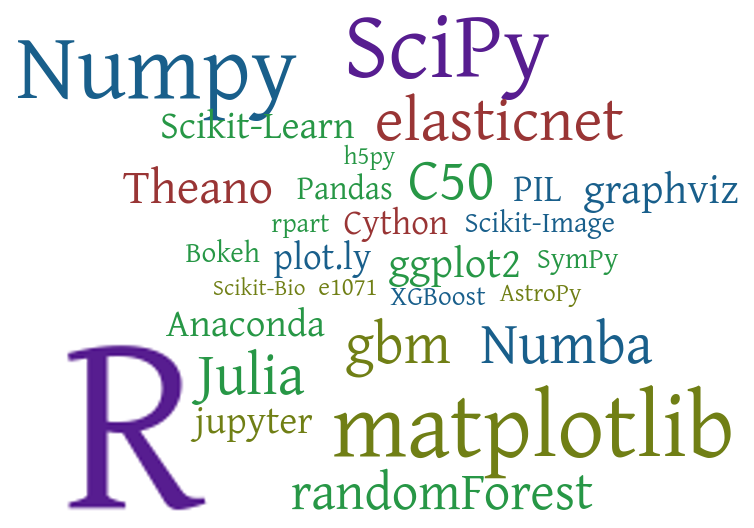
\includegraphics[height=3.5 cm]{statistical-software.png}
\vspace{0.125 cm}
\end{center}

\vspace{-0.35 cm}
\begin{uncoverenv}<2->
\begin{itemize}
\item Mostly natively compiled, driven by high-level languages.
\item Primary customer is the laptop data analysis.
\end{itemize}
\end{uncoverenv}

\column{0.5\linewidth}
\begin{center}
\textcolor{darkblue}{\Large \underline{Big Data}}

\vspace{0.25 cm}
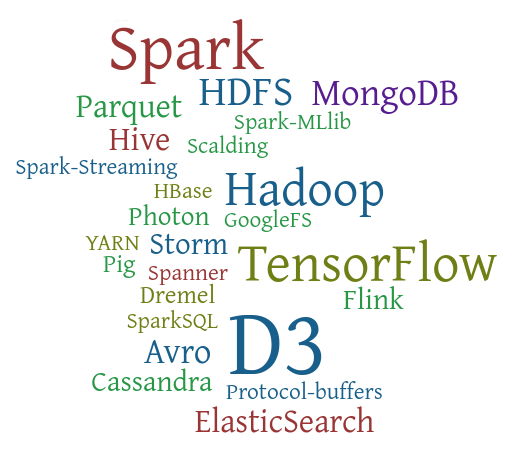
\includegraphics[height=3.75 cm]{bigdata-software.png}
\end{center}

\vspace{-0.35 cm}
\begin{uncoverenv}<3->
\begin{itemize}
\item Mostly Java/Spark/Clojure.
\item More emphasis on scale-out than single-processor speed.
\item Datasets assumed to be {\it big.}
\end{itemize}
\end{uncoverenv}

\end{columns}
\end{frame}

\begin{frame}{A third you may not have heard about}
\vspace{0.5 cm}
\begin{center}
\textcolor{darkblue}{\Large \underline{High Energy Physics (HEP)}}

\vspace{0.25 cm}
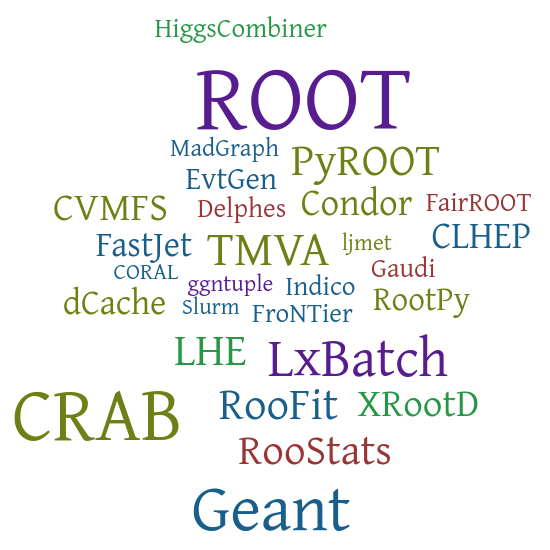
\includegraphics[height=6 cm]{hep-software.png}
\end{center}
\end{frame}

\begin{frame}{A third you may not have heard about}
\vspace{0.25 cm}
\begin{columns}
\column{0.5\linewidth}
\begin{center}
\textcolor{darkblue}{\Large \underline{High Energy Physics (HEP)}}

\vspace{0.25 cm}
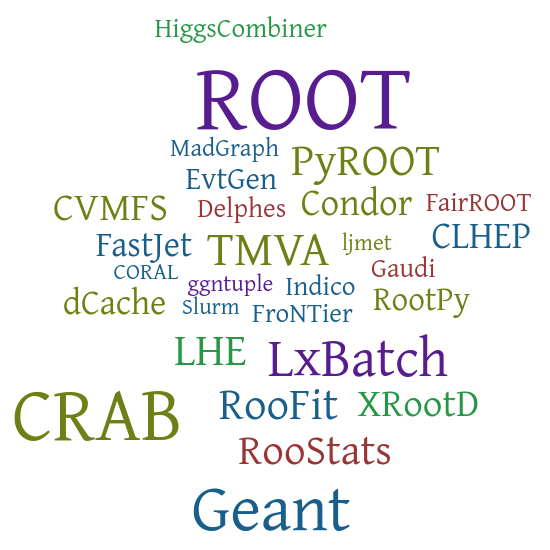
\includegraphics[height=6 cm]{hep-software.png}
\end{center}

\column{0.5\linewidth}
\begin{itemize}
\item Natively compiled, optimized for single-processor throughput.
\item<2-> {\it Throughput,} not speed: this is not High Performance Computing (HPC).
\item<3-> Datasets have always been ``big'' 
\begin{itemize}
\item<3-> SPS in 1980's: $\sim$100~GB per year
% https://www.researchgate.net/publication/275209564_UA1_Data-acquisition_System 1.6 MB/event? (``raw'')
% https://cern.ch/delfino/Generic%20LHC%20Computing%202000.ppt 0.1 MB/event (probably after processing)
% http://cerncourier.com/cws/article/cern/28849
\item<4-> LHC today: $\sim$25~PB per year
% http://www.lhc-closer.es/taking_a_closer_look_at_lhc/0.lhc_data_analysis
% https://home.cern/about/updates/2013/02/cern-data-centre-passes-100-petabytes
\end{itemize}
\end{itemize}

\vspace{0.2 cm}
\hfill \only<1-2>{
\includegraphics[width=0.87\linewidth]{blank.png}}\only<3>{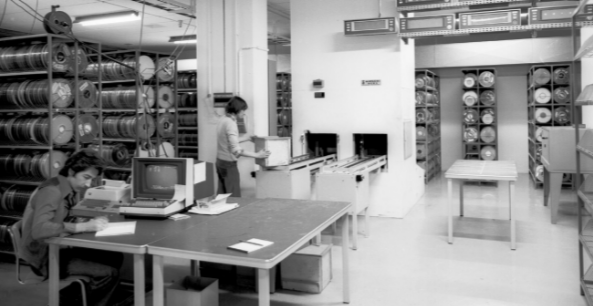
\includegraphics[width=0.87\linewidth]{tapes1.png}}\only<4>{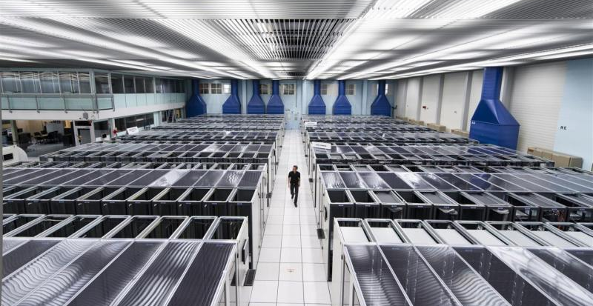
\includegraphics[width=0.87\linewidth]{cerncomputing.png}}
\vspace{-0.2 cm}
\end{columns}
\end{frame}

\begin{frame}{}
\begin{center}
\Large For decades, HEP seemed to be the only field with these problems.

\vspace{0.5 cm}
\uncover<2->{That is no longer true.}
\end{center}

\begin{columns}
\column{0.4\linewidth}
\begin{uncoverenv}<3->
\begin{itemize}
\item HEP software needs clearly overlap with the Scipy/R/ Scikit-Learn world and the Spark/Hadoop/NoSQL world. \\ \mbox{ }
\end{itemize}
\end{uncoverenv}

\column{0.4\linewidth}
\begin{uncoverenv}<4->
\begin{itemize}
\item Individual physicists and projects like DIANA-HEP \\ (my job) are starting to explore and develop these connections.
\end{itemize}
\end{uncoverenv}

\end{columns}
\vspace{-1.5 cm}
\end{frame}

\begin{frame}{}
\vspace{1 cm}
\begin{center}
\large Considering how much has been developed on both sides of the divide, \\ small ``glue projects'' connecting them can make a big difference.
\end{center}

\vspace{1 cm}
\mbox{\hspace{-1.2 cm}}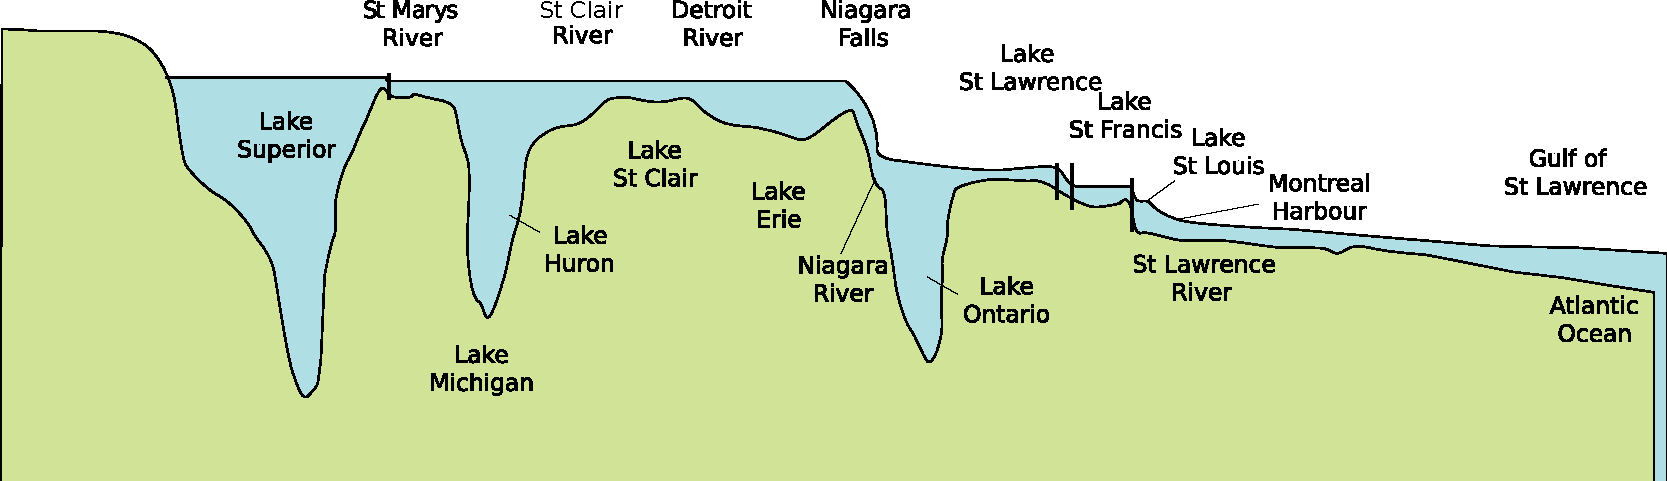
\includegraphics[width=1.16\linewidth]{great_lakes_levels.pdf}
\vspace{-1 cm}
\end{frame}

\begin{frame}{Taxonomy of the Revolution}
\vspace{0.25 cm}
\begin{columns}[t]
\column{0.33\linewidth}
\textcolor{darkblue}{\underline{Type I:}} HEP software that serves {\it the same function} as software in the wider community.

\begin{uncoverenv}<2->
\begin{center}

\includegraphics[height=1.5 cm]{stamp_replace.png}
\end{center}

Wider community has better resources for
\begin{itemize}
\item maintaining code
\item catching bugs
\item revising bad designs.
\end{itemize}
\end{uncoverenv}

\column{0.33\linewidth}
\textcolor{darkblue}{\underline{Type II:}} Domain-specific software for HEP applications. For example, ``HiggsCombiner.''

\begin{uncoverenv}<3->
\begin{center}

\includegraphics[height=1.5 cm]{stamp_keep.png}
\end{center}

Obviously. This really is a unique problem.
\end{uncoverenv}

\column{0.33\linewidth}
\textcolor{darkblue}{\underline{Type III:}} HEP software and concepts that would benefit the wider community. \\ \mbox{ }

\begin{uncoverenv}<4->
\begin{center}

\includegraphics[height=1.5 cm]{stamp_promulgate.png}
\end{center}

Cultural exchange goes both ways.
\end{uncoverenv}
\end{columns}
\end{frame}

\begin{frame}{Topic of this talk}
\begin{center}
\Large Histograms are an example of \textcolor{darkblue}{Type III}:

\vspace{0.5 cm}
HEP has a unique and useful approach.
\end{center}
\end{frame}

\begin{frame}{Statistical definition of a histogram}
\vspace{0.75 cm}
A {\bf histogram} is an approximation of a distribution, formed by partitioning a sample by one of its features and counting how many items fall in each partition.

\vspace{0.25 cm}
The partitions are called {\bf bins}, and the content of each bin may be represented as the total count or the average density in that partition. \textcolor{gray}{[Start philosophical argument here.]}

\begin{center}
\only<1>{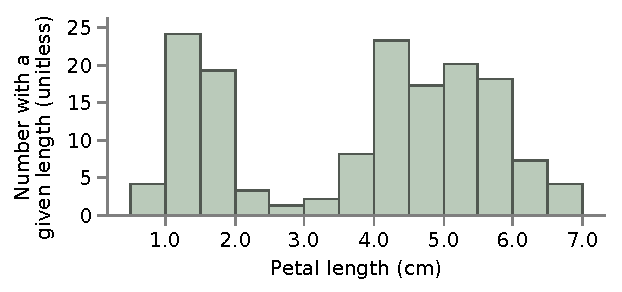
\includegraphics[width=0.7\linewidth]{Iris_Petal_Length_Histogram.pdf}}
\only<2>{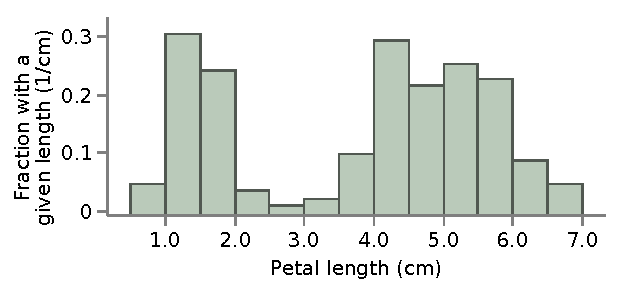
\includegraphics[width=0.7\linewidth]{Iris_Petal_Length_Histogram-2.pdf}}
\end{center}
\end{frame}

\begin{frame}[fragile]{Gallery of histogram APIs: non-HEP}
\vspace{0.25 cm}
\begin{columns}
\column{0.50\linewidth}
\begin{description}
\item[R:]

\begin{lstlisting}
hist(x, breaks =
   "Sturges", ...)
\end{lstlisting}

{\tt x} input data samples \\
{\tt breaks} binning strategy

\item[Numpy:]

\begin{lstlisting}
numpy.histogram(a, bins = 10, ...)
\end{lstlisting}

{\tt a} input data samples \\
{\tt bins} binning strategy

\item[Pandas:]

\begin{lstlisting}
DataFrame.hist(data, bins = 10, ...)
\end{lstlisting}

{\tt data} input data samples \\
{\tt bins} binning strategy
\end{description}

\column{0.51\linewidth}
\begin{description}
\item[Spark:]

\begin{lstlisting}
DoubleRDDFunctions.histogram(buckets: Array[Double])
\end{lstlisting}

{\tt this} input data samples \\
{\tt buckets} binning strategy

\item[Mathematica:]

\begin{lstlisting}
Histogram[data, hspec]
\end{lstlisting}

{\tt data} input data samples \\
{\tt hspec} binning strategy

\item[MATLAB:]

\begin{lstlisting}
histogram(X, nbins)
\end{lstlisting}

{\tt X} input data samples \\
{\tt nbins} binning strategy

\end{description}
\end{columns}

\begin{uncoverenv}<2->
\vspace{-5 cm}
\begin{center}
\fcolorbox{black}{white}{\begin{minipage}{0.85\linewidth}
\vspace{0.75 cm}
\centering They all require {\it all} of the input data before giving you a histogram.
\vspace{0.75 cm}
\end{minipage}}
\end{center}
\vspace{5 cm}
\end{uncoverenv}
\end{frame}

\begin{frame}[fragile]{HEP histograms are different}
HEP software (HBOOK, PAW, ROOT, HippoDraw, AIDA, \ldots) treats histograms as {\it fillable containers.}

\begin{center}
\fbox{\begin{minipage}{0.6\linewidth}
\vspace{0.3 cm}
\begin{onlyenv}<1>
\vspace{0.5\baselineskip}
\hfill \begin{minipage}{0.9\linewidth}
\ttfamily\small
h = Histogram(numBins, \\
\mbox{\hspace{1.5 cm}}lowEdge, highEdge) \\
\\
for x in data: \\
\mbox{\hspace{0.75 cm}}h.fill(x) \\
\\
h.plot()
\end{minipage}
\vspace{0.5\baselineskip}
\end{onlyenv}
%% \begin{onlyenv}<2->
%% \hfill \begin{minipage}{0.9\linewidth}
%% \ttfamily\small
%% h = Histogram(numBins, \\
%% \mbox{\hspace{1.5 cm}}lowEdge, highEdge, "pt") \\
%% \\
%% for mu in muons: \\
%% \mbox{\hspace{0.75 cm}}pt = sqrt(mu.px**2 + mu.py**2) \\
%% \mbox{\hspace{0.75 cm}}h.fill(pt) \\
%% \\
%% h.plot()
%% \end{minipage}
%% \end{onlyenv}
\vspace{0.3 cm}
\end{minipage}}
\end{center}

API presumes the dataset is too big for a single function call.

\vspace{0.25 cm}
{\it Intrinsically} single-pass (implementation can't pre-scan to set bin width or range).

\vspace{-0.5 cm}
\end{frame}

\begin{frame}{Everything is made out of histograms}
\vspace{0.5 cm}
\mbox{\hspace{-1.1 cm}
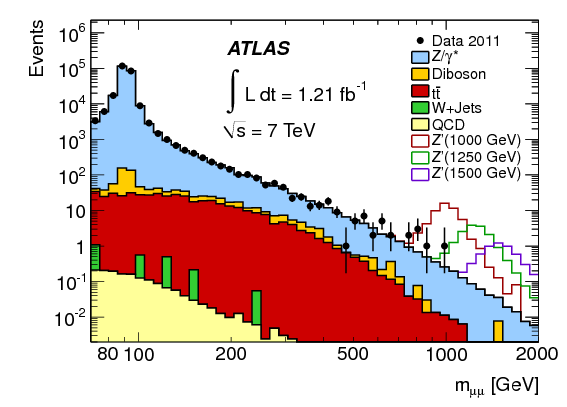
\includegraphics[height=1.8cm]{dileptons_fig_01b_mumu.png}
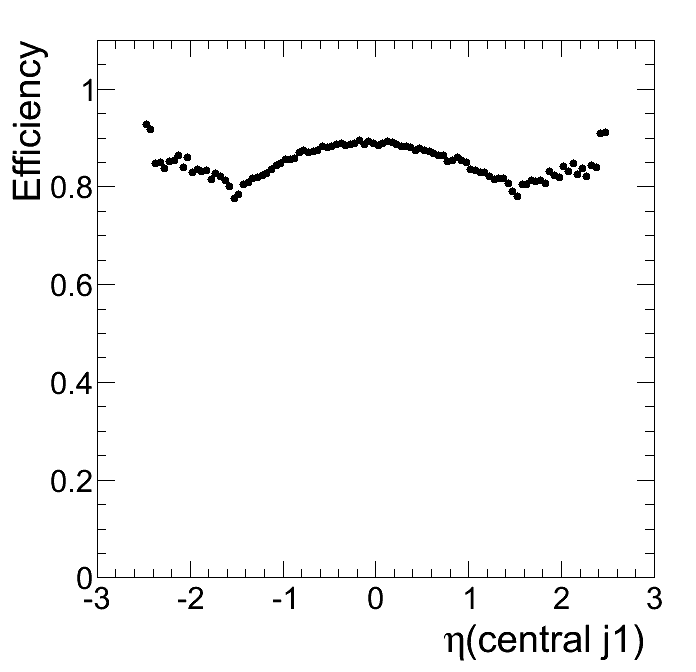
\includegraphics[height=1.8cm]{efficiency.png}
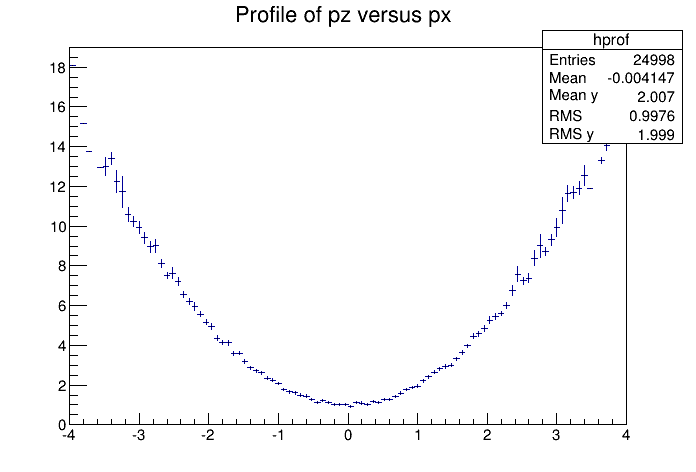
\includegraphics[height=1.8cm]{profile_plot.png}
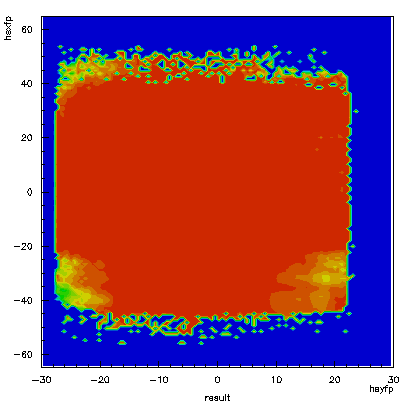
\includegraphics[height=1.8cm]{efficiency_2d.png}
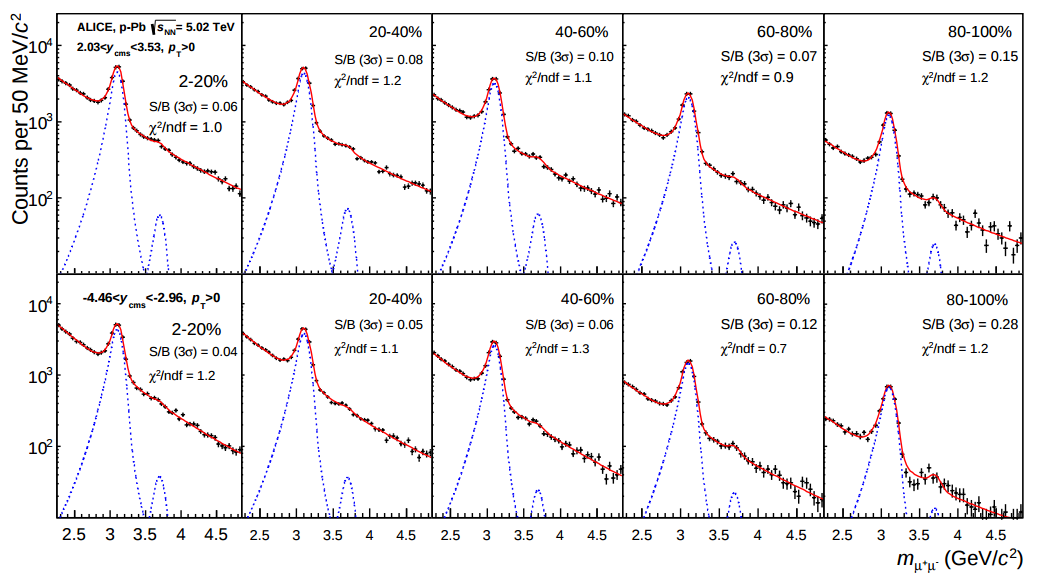
\includegraphics[height=1.8cm]{histograms_of_histograms.png}
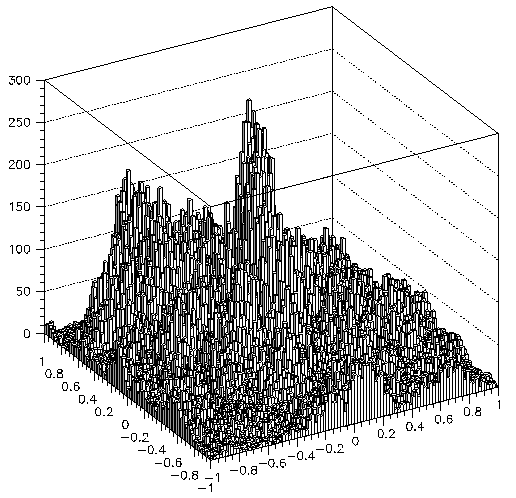
\includegraphics[height=1.8cm]{lego_plot.png}
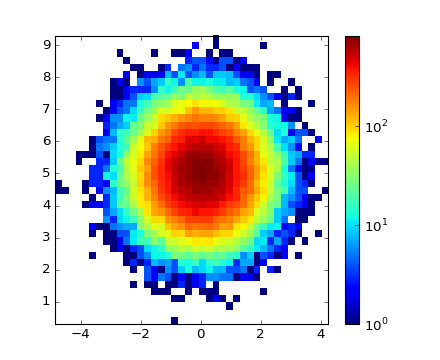
\includegraphics[height=1.8cm]{two_dimensional.png}}

\vspace{0.5 cm}
\begin{center}
\begin{minipage}{0.9\linewidth}
\Large Histograms are the basic unit of HEP data analysis, used to make almost everything else. Analogous to

\vspace{0.5 cm}
\hspace{0.5 cm}\begin{minipage}{0.5\linewidth}
\begin{itemize}
\item lists in LISP
\item dictionaries in Python
\item data.frames in R
\end{itemize}
\end{minipage}
\end{minipage}
\end{center}
\end{frame}

\begin{frame}{Examples (only one of which is really a histogram)}
\vspace{0.5 cm}
\begin{columns}
\column{0.33\linewidth}
\mbox{ } \hfill \hfill \hfill \textcolor{darkblue}{Stacked histograms} \hfill \mbox{ }

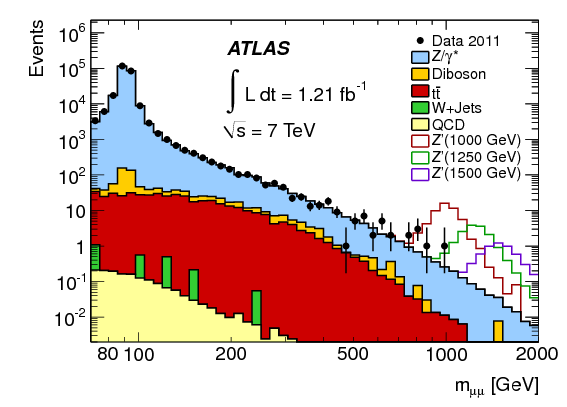
\includegraphics[height=3.5 cm]{dileptons_fig_01b_mumu.png}

Represents contributions from different samples to a total histogram.

\vspace{0.25 cm}
\begin{minipage}{\linewidth}
\scriptsize \textcolor{gray}{Constructed by cumulatively filling a series of histograms and overlaying them in reverse order.}
\end{minipage}

\column{0.33\linewidth}
\mbox{ } \hfill \hfill \textcolor{darkblue}{Efficiency plot} \hfill \mbox{ }

\mbox{ } \hfill 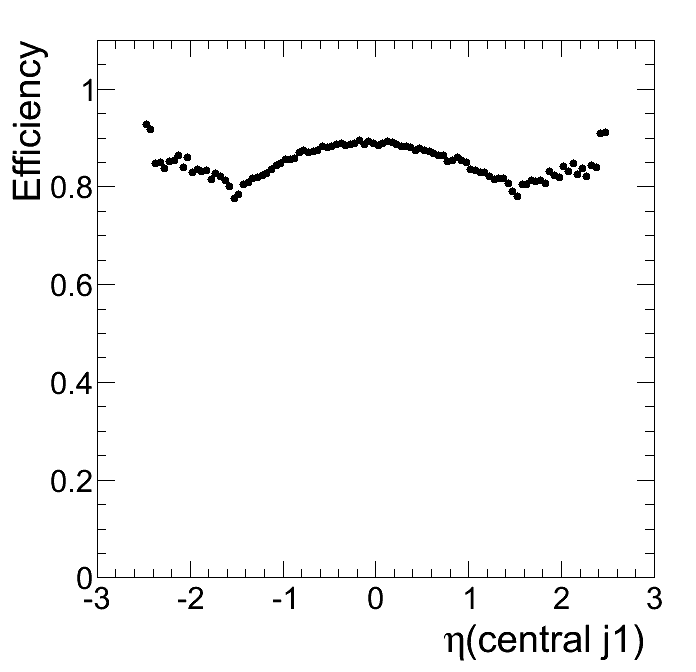
\includegraphics[height=3.5 cm]{efficiency.png} \hfill \mbox{ }

Represents the probability of passing a filter versus some variable.

\vspace{0.25 cm}
\begin{minipage}{\linewidth}
\scriptsize \textcolor{gray}{Constructed by filling two histograms, one with the filter, the other without, and dividing them bin-by-bin.}
\end{minipage}

\column{0.33\linewidth}
\mbox{ } \hfill \textcolor{darkblue}{Profile plot} \hfill \mbox{ }

\mbox{\hspace{-0.25 cm}}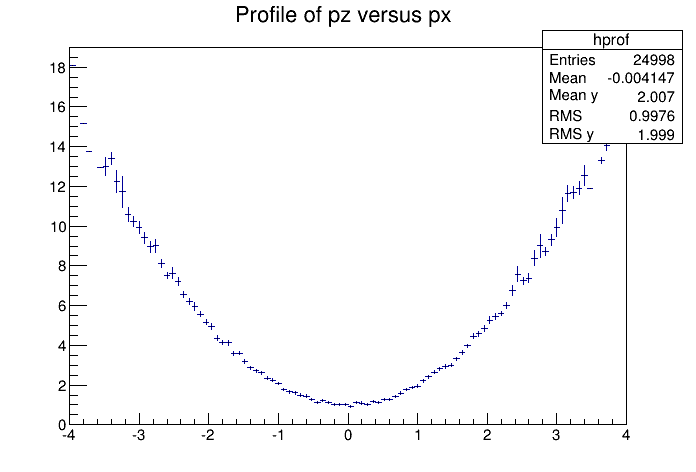
\includegraphics[height=3.5 cm]{profile_plot.png}

Represents a marginal projection of the dataset with errors on the mean.

\vspace{0.25 cm}
\begin{minipage}{\linewidth}
\scriptsize \textcolor{gray}{Constructed by filling $\sum_i y_i$ and $\sum_i {y_i}^2$ separately and doing the appropriate transformations bin-by-bin.}
\end{minipage}
\end{columns}
\end{frame}

\begin{frame}{The problem with this API}
\vspace{0.65 cm}
\textcolor{darkblue}{Domain-specific knowledge enters in two different places: histogram-construction and histogram-filling.}

\begin{center}
\begin{minipage}{0.8\linewidth}
\vspace{0.25 cm}
$\left.\mbox{\rotatebox{90}{\hspace{-0.9 cm}construction}\hspace{0.15 cm}}\right\{\begin{array}{l}\mbox{\ttfamily\small job[N].h = Histogram(numBins, lowEdge, highEdge)} \\ \hspace{2.3 cm}\mbox{\textcolor{darkblue}{\# binning requires knowledge of the problem domain}}\end{array}$

\vspace{0.25 cm}
$\left.\mbox{\rotatebox{90}{\hspace{-0.65 cm}\hspace{0.35 cm}filling\hspace{0.35 cm}}}\hspace{0.1 cm}\right\{\begin{array}{l}\mbox{\ttfamily\small for event in job[N].physicsEvents:} \\ \mbox{\ttfamily\small \hspace{0.75 cm}job[N].h.fill(event.whatToPlot())} \\ \hspace{2.3 cm}\mbox{\textcolor{darkblue}{\# {\ttfamily\small whatToPlot()} requires knowledge of the problem domain}}\end{array}$

\vspace{0.25 cm}
$\left.\mbox{\rotatebox{90}{\hspace{-0.5 cm}merging}}\hspace{0.1 cm}\right\{\begin{array}{l}\mbox{\ttfamily\small h = job[0].h + job[1].h + job[2].h + ...}\end{array}$
\end{minipage}
\end{center}
\end{frame}

\begin{frame}[fragile]{Specifically, in Spark\ldots}
\vspace{0.5 cm}
\begin{columns}
\column{0.5\linewidth}

\textcolor{darkblue}{Imperative analysis script}
\small
\begin{minted}{python}
x = Histogram(100, -5.0, 5.0)

for event in events:
    x.fill(event.calcX())

x.plot()
\end{minted}

\column{0.52\linewidth}
\textcolor{darkblue}{Spark equivalent}
\small
\begin{minted}{python}
x = events.aggregate(
    monoid_zero(),
    lambda h, event:
        monoid_successor(h, event),
    lambda h1, h2:
        monoid_add(h1, h2))

x.plot()
\end{minted}
\end{columns}
\end{frame}

\begin{frame}[fragile]{Specifically, in Spark\ldots}
\vspace{0.5 cm}
\begin{columns}
\column{0.5\linewidth}

\textcolor{darkblue}{Imperative analysis script}
\small
\begin{minted}{python}
x = Histogram(100, -5.0, 5.0)

for event in events:
    x.fill(event.calcX())

x.plot()
\end{minted}

\column{0.52\linewidth}
\textcolor{darkblue}{Spark equivalent}
\small
\begin{minted}{python}
x = events.aggregate(
    Histogram(100, -5.0, 5.0),
    lambda h, event:
        h.fill(event.calcX()),
    lambda h1, h2:
        h1 + h2)

x.plot()
\end{minted}
\end{columns}
\end{frame}

\begin{frame}[fragile]{Specifically, in Spark\ldots}
\vspace{0.5 cm}
\begin{columns}
\column{0.5\linewidth}

\textcolor{darkblue}{Imperative analysis script}
\small
\begin{minted}{python}
x = Histogram(100, -5.0, 5.0)
y = Histogram(100, -5.0, 5.0)

for event in events:
    x.fill(event.calcX())
    y.fill(event.calcY())

x.plot()
y.plot()
\end{minted}

\column{0.52\linewidth}
\textcolor{darkblue}{Spark equivalent}
\small
\begin{minted}{python}
x, y = events.aggregate(
    (Histogram(100, -5.0, 5.0),
     Histogram(100, -5.0, 5.0)),
    lambda hs, event: (
        hs[0].fill(event.calcX()),
        hs[1].fill(event.calcY())),
    lambda hs1, hs2: (
        hs1[0] + hs2[0],
        hs1[1] + hs2[1]))

x.plot()
y.plot()
\end{minted}
\end{columns}
\end{frame}

\begin{frame}[fragile]{Specifically, in Spark\ldots}
\vspace{0.5 cm}
\begin{columns}
\column{0.5\linewidth}

\textcolor{darkblue}{Imperative analysis script}
\small
\begin{minted}{python}
x = Histogram(100, -5.0, 5.0)
y = Histogram(100, -5.0, 5.0)
z = Histogram(100, -5.0, 5.0)

for event in events:
    x.fill(event.calcX())
    y.fill(event.calcY())
    z.fill(event.calcZ())

x.plot()
y.plot()
z.plot()
\end{minted}

\column{0.52\linewidth}
\textcolor{darkblue}{Spark equivalent}
\small
\begin{minted}{python}
x, y, z = events.aggregate(
    (Histogram(100, -5.0, 5.0),
     Histogram(100, -5.0, 5.0),
     Histogram(100, -5.0, 5.0)),
    lambda hs, event: (
        hs[0].fill(event.calcX()),
        hs[1].fill(event.calcY()),
        hs[2].fill(event.calcZ())),
    lambda hs1, hs2: (
        hs1[0] + hs2[0],
        hs1[1] + hs2[1],
        hs1[2] + hs2[2]))

x.plot()
y.plot()
z.plot()
\end{minted}
\end{columns}
\end{frame}

\begin{frame}[fragile]{Solution: go functional}
\vspace{0.5 cm}
\begin{center}
\fbox{\begin{minipage}{0.85\linewidth}
\vspace{0.25 cm}
\ttfamily\small\hspace{0.25 cm} h = Histogram(numBins, lowEdge, highEdge, \textbf{fillRule})
\vspace{0.25 cm}
\end{minipage}}
\end{center}

where {\ttfamily\small\textbf{fillRule}} is a function : {\it data} $\to$ $\mathbb{R}$ that specifies how to get the binnable feature from the input dataset.

\begin{uncoverenv}<2->
\vspace{0.5 cm}
All domain-specific knowledge is in the binning and the {\ttfamily\small\textbf{fillRule}}. The filling function may now be generic (and automated).

\begin{center}
\fbox{\begin{minipage}{0.85\linewidth}
\vspace{0.25 cm}
\ttfamily\small\hspace{0.25 cm} h.fill(datum) \hspace{1 cm}\textcolor{gray}{\textit{\# calls fillRule(datum) internally}}
\vspace{0.25 cm}
\end{minipage}}
\end{center}
\end{uncoverenv}

\begin{uncoverenv}<3->
\vspace{0.25 cm}
(In a {\it purely} functional environment, {\ttfamily\small hnew = hold.filled(datum)}.)
\end{uncoverenv}
\end{frame}

\begin{frame}[fragile]{What this looks like in Spark}
\begin{columns}
\column{0.46\linewidth}
\small
\begin{minted}{python}
# Define increment and combine
# as reusable library functions.

def increment(h, event):
    h.fill(event)
    return h

def combine(h1, h2):
    return h1 + h2

x = events.aggregate(
    Histogram(100, -5.0, 5.0,
       lambda ev: ev.calcX()),
    increment,
    combine)


x.plot()
\end{minted}

\column{0.59\linewidth}
\begin{uncoverenv}<2->
\small
\begin{minted}{python}
class Package:     # also in the library
  def __init__(self, **hs):
      self.hs = hs
  def fill(self, datum):
      for h in self.hs.values():
          h.fill(datum)
  def __add__(self, other):
      return {n: self.hs[n] + other.hs[n]
                        for n in self.hs}

pkg = events.aggregate(Package(
        x = Histogram(100, -5.0, 5.0,
                lambda ev: ev.calcX()),
        y = Histogram(100, -5.0, 5.0,
                lambda ev: ev.calcY()))
    increment, combine)

pkg.hs["x"].plot()
\end{minted}
\end{uncoverenv}
\end{columns}
\end{frame}

\begin{frame}{}
\begin{center}
\Large This ``\textcolor{blue}{\ttfamily \textbf{Package}}'' has the same interface as a \textcolor{blue}{\ttfamily \textbf{Histogram}}, namely the \textcolor{blue}{\ttfamily \textbf{fill}} and \textcolor{blue}{\ttfamily \textbf{+}} methods.
\end{center}
\end{frame}

\begin{frame}{Elaboration: go compositional}
\begin{center}
\begin{minipage}{0.8\linewidth}
\Large
Generic aggregators:
\vspace{0.25 cm}
\begin{description}
\item[Count] number of times ``fill'' is called
\item[Bin$\lbrack\,\cdot\,\rbrack$] partitions according to fillRule, passes data to {\it one} subaggregator
\item[Label$\lbrack\,\cdot\,\rbrack$] passes data to {\it all} named subaggregators
\end{description}

\vspace{0.75 cm}
\textcolor{gray}{\normalsize (Naming convention: all aggregators are verbs.)}
\end{minipage}
\end{center}
\end{frame}

%% \begin{frame}[fragile]{}
%% \vspace{1.5 cm}
%% \textcolor{darkblue}{\Large Spark example in Python:}
%% \small
%% \begin{minted}{python}
%% pkg = events.aggregate(
%%     Label(x = Bin(100, -5.0, 5.0, lambda ev: ev.calcX(), Count()),
%%           y = Bin(100, -5.0, 5.0, lambda ev: ev.calcY(), Count()),
%%           z = Bin(100, -5.0, 5.0, lambda ev: ev.calcZ(), Count())),
%%     increment, combine)
%% \end{minted}

%% \vspace{0.75 cm}
%% \textcolor{darkblue}{\Large Spark example in Scala:}
%% \small
%% \begin{minted}{scala}
%% val pkg = events.aggregate(
%%     Label(x -> Bin(100, -5.0, 5.0, {ev: Event => ev.calcX}, Count()),
%%           y -> Bin(100, -5.0, 5.0, {ev: Event => ev.calcY}, Count()),
%%           z -> Bin(100, -5.0, 5.0, {ev: Event => ev.calcZ}, Count())))
%%     (new Increment, new Combine)
%% \end{minted}

%% \normalsize Type parameters inferred from arguments, propagated to \textcolor{blue}{\ttfamily\small \textbf{Increment}} and \textcolor{blue}{\ttfamily\small \textbf{Combine}}.
%% \end{frame}

\begin{frame}[fragile]{With the right set of aggregators, you can do anything}
\vspace{0.5 cm}
\begin{columns}
\column{0.5\linewidth}
\small
\textcolor{darkblue}{\normalsize Histograms:}
\begin{minted}{python}
Bin(num, low, high, fillRule,
  Count())
\end{minted}

\vspace{0.25 cm}
\textcolor{darkblue}{\normalsize Two-dimensional histograms:}
\begin{minted}{python}
Bin(xnum, xlow, xhigh, xfill,
  Bin(ynum, ylow, yhigh, yfill,
    Count()))
\end{minted}

\vspace{0.25 cm}
\textcolor{darkblue}{\normalsize Profile plots:}
\begin{minted}{python}
Bin(xnum, xlow, xhigh, xfill,
  Deviate(yfill))
\end{minted}

{\normalsize where {\ttfamily\small Deviate} computes a mean and standard deviation.}

\column{0.5\linewidth}
\small
\textcolor{darkblue}{\normalsize Mix and match binning methods:}
\begin{minted}{python}
IrregularlyBin([-2.4, -2.1, -1.5,
    0.0, 1.5, 2.1, 2.4],
  filleta,
  Bin(314, -3.14, 3.14, fillphi,
    Count()))

SparselyBin(0.01, filleta,
  Bin(314, -3.14, 3.14, fillphi,
    Count()))

Categorize(fillByName,
  Bin(314, -3.14, 3.14, fillphi,
    Count()))
\end{minted}
\end{columns}
\end{frame}

\begin{frame}[fragile]{With the right set of aggregators, you can do anything}
\vspace{0.75 cm}
\small
\textcolor{darkblue}{\normalsize Create complex trees, detailing exactly what you want to aggregate:}
\begin{minted}{python}
    Bin(xnum, xlow, xhigh, lambda datum: datum.x,
      Branch(Count(),
             Minimize(lambda datum: datum.y),
             Maximize(lambda datum: datum.y),
             Average(lambda datum: datum.y),
             Sum(lambda datum: datum.weight),
             Sum(lambda datum: datum.weight**2)))
\end{minted}

\vspace{0.25 cm}
\begin{center}
\begin{minipage}{0.8\linewidth}
Now each bin in {\ttfamily\small x} contains
\begin{columns}
\column{0.05\linewidth}
\column{0.45\linewidth}
\begin{itemize}
\item number of entries,
\item minimum {\ttfamily\small y} value,
\item maximum {\ttfamily\small y} value,
\end{itemize}

\column{0.45\linewidth}
\begin{itemize}
\item average of {\ttfamily\small y},
\item sum of weights,
\item sum of weights squared.
\end{itemize}
\column{0.05\linewidth}
\end{columns}

\end{minipage}
\end{center}
\end{frame}

\begin{frame}[fragile]{With the right set of aggregators, you can do anything}
\begin{center}
\begin{minipage}{0.9\linewidth}
\small
\textcolor{darkblue}{\normalsize High-level interface to common patterns:}
\begin{minted}{python}
    Fraction(cut, Bin(numBins, lowEdge, highEdge, fillRule))
\end{minted}

{\normalsize to make a ratio plot,}

\begin{minted}{python}
    Stack(cuts, Bin(numBins, lowEdge, highEdge, fillRule))
\end{minted}

{\normalsize to make stacked histograms.}

\vspace{0.75 cm}
{\normalsize Guarantees that the numerator/denominator or the stacked items have \mbox{consistent} binning for the bin-by-bin division or sum.}
\end{minipage}
\end{center}
\end{frame}

\begin{frame}{}
\hspace{-1 cm}\mbox{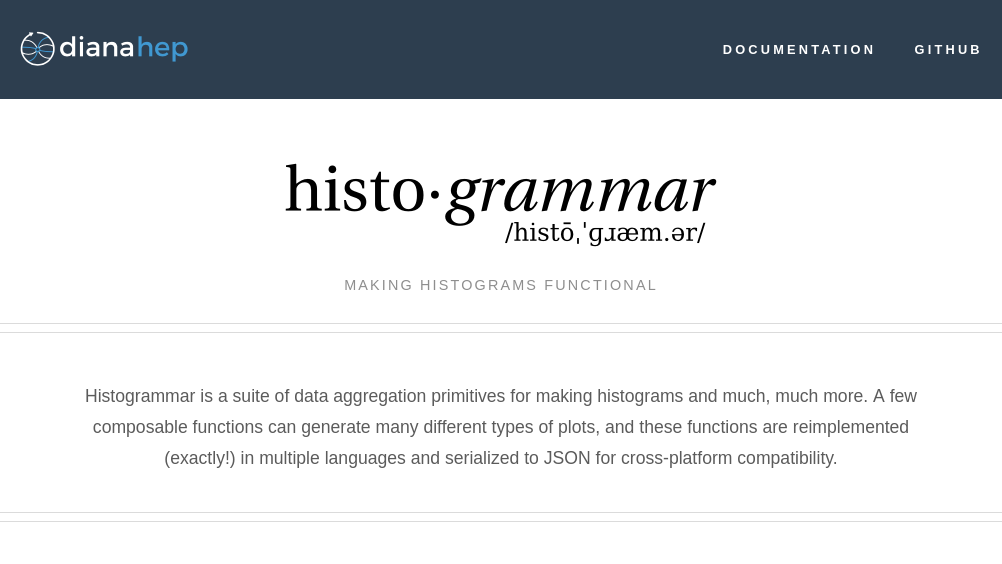
\includegraphics[width=16 cm]{frontpage.png}\hspace{-5 cm}}
\end{frame}

\begin{frame}{Histogrammar}
\large Histogrammar is a suite of composable aggregators with

\vspace{0.3 cm}
\begin{itemize}\setlength{\itemsep}{0.3 cm}
\item<2-> a language-independent specification,
\item<3-> several language versions (Python and Scala are the most complete),
\item<4-> an interchangeable JSON format,
\item<5-> multiple filling back-ends: ``normal,'' SparkSQL optimizations, Numpy optimizations, JIT-compilation, GPU (CUDA) code generation\ldots
\item<6-> no built-in plotting: Matplotlib, Bokeh, ROOT as front-ends.
\end{itemize}
\end{frame}

\begin{frame}{User's perspective}
\vspace{0.5 cm}
\begin{center}
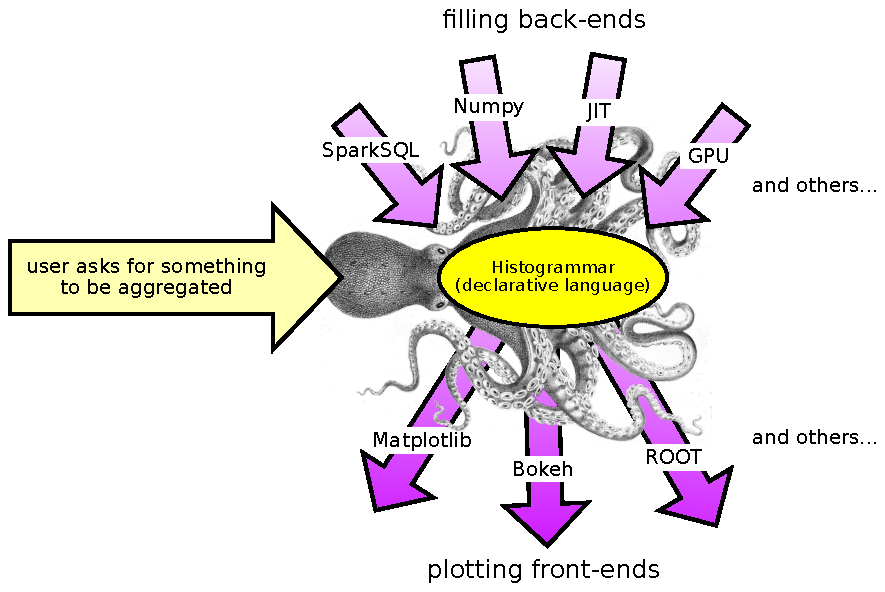
\includegraphics[width=0.75\linewidth]{front-back-ends.pdf}
\end{center}
\end{frame}

\begin{frame}{Current coverage}
\vspace{0.4 cm}
\renewcommand{\arraystretch}{1.1}
\scriptsize
\mbox{\hspace{-0.75 cm}}\begin{tabular}{l c c c c c c c c c c c c}
Aggregator        & Scala                      & JVM-JIT & Python                     & Numpy                      & C-JIT                   & GPU                        & C++11                      & Julia & R & Javascript \\\hline\hline
Count             & \cellcolor{yellow!50}DONE  &         & \cellcolor{yellow!50}DONE  & \cellcolor{yellow!50}DONE  & \cellcolor{yellow!50}DONE  & \cellcolor{yellow!50}DONE  & \cellcolor{red!25}trial    & \cellcolor{yellow!50}DONE & & \\
Sum               & \cellcolor{yellow!50}DONE  &         & \cellcolor{yellow!50}DONE  & \cellcolor{yellow!50}DONE  & \cellcolor{yellow!50}DONE  & \cellcolor{yellow!50}DONE  & \cellcolor{red!25}trial    & \cellcolor{yellow!50}DONE & & \\
Average           & \cellcolor{yellow!50}DONE  &         & \cellcolor{yellow!50}DONE  & \cellcolor{yellow!50}DONE  & \cellcolor{yellow!50}DONE  & \cellcolor{yellow!50}DONE  &                            & \cellcolor{yellow!50}DONE & & \\
Deviate           & \cellcolor{yellow!50}DONE  &         & \cellcolor{yellow!50}DONE  & \cellcolor{yellow!50}DONE  & \cellcolor{yellow!50}DONE  & \cellcolor{yellow!50}DONE  &                            & \cellcolor{yellow!50}DONE & & \\
Minimize          & \cellcolor{yellow!50}DONE  &         & \cellcolor{yellow!50}DONE  & \cellcolor{yellow!50}DONE  & \cellcolor{yellow!50}DONE  & \cellcolor{yellow!50}DONE  &                            & \cellcolor{yellow!50}DONE & & \\
Maximize          & \cellcolor{yellow!50}DONE  &         & \cellcolor{yellow!50}DONE  & \cellcolor{yellow!50}DONE  & \cellcolor{yellow!50}DONE  & \cellcolor{yellow!50}DONE  &                            & \cellcolor{yellow!50}DONE & & \\
Bag               & \cellcolor{green!25}DONE   &         & \cellcolor{green!25}DONE   & \cellcolor{green!25}DONE   & \cellcolor{green!25}DONE   & growable?                  &                            & \cellcolor{green!25}DONE  & & \\\hline
Bin               & \cellcolor{yellow!50}DONE  &         & \cellcolor{yellow!50}DONE  & \cellcolor{yellow!50}DONE  & \cellcolor{yellow!50}DONE  & \cellcolor{yellow!50}DONE  & \cellcolor{red!25}trial    & \cellcolor{yellow!50}DONE & & \\
SparselyBin       & \cellcolor{yellow!50}DONE  &         & \cellcolor{yellow!50}DONE  & \cellcolor{yellow!50}DONE  & \cellcolor{yellow!50}DONE  & growable?                  &                            &                           & & \\
CentrallyBin      & \cellcolor{yellow!50}DONE  &         & \cellcolor{yellow!50}DONE  & \cellcolor{yellow!50}DONE  & \cellcolor{yellow!50}DONE  & \cellcolor{yellow!50}DONE  &                            &                           & & \\
IrregularlyBin    & \cellcolor{yellow!50}DONE  &         & \cellcolor{yellow!50}DONE  & \cellcolor{yellow!50}DONE  & \cellcolor{yellow!50}DONE  & \cellcolor{yellow!50}DONE  &                            &                           & & \\
Categorize        & \cellcolor{yellow!50}DONE  &         & \cellcolor{yellow!50}DONE  & \cellcolor{yellow!50}DONE  & \cellcolor{yellow!50}DONE  & growable?                  &                            &                           & & \\
Fraction          & \cellcolor{yellow!50}DONE  &         & \cellcolor{yellow!50}DONE  & \cellcolor{yellow!50}DONE  & \cellcolor{yellow!50}DONE  & \cellcolor{yellow!50}DONE  &                            &                           & & \\
Stack             & \cellcolor{yellow!50}DONE  &         & \cellcolor{yellow!50}DONE  & \cellcolor{yellow!50}DONE  & \cellcolor{yellow!50}DONE  & \cellcolor{yellow!50}DONE  &                            &                           & & \\
Select            & \cellcolor{yellow!50}DONE  &         & \cellcolor{yellow!50}DONE  & \cellcolor{yellow!50}DONE  & \cellcolor{yellow!50}DONE  & \cellcolor{yellow!50}DONE  & \cellcolor{red!25}trial    &                           & & \\\hline
Label             & \cellcolor{yellow!50}DONE  &         & \cellcolor{yellow!50}DONE  & \cellcolor{yellow!50}DONE  & \cellcolor{yellow!50}DONE  & \cellcolor{yellow!50}DONE  &                            &                           & & \\
UntypedLabel      & \cellcolor{yellow!50}DONE  &         & \cellcolor{yellow!50}DONE  & \cellcolor{yellow!50}DONE  & \cellcolor{yellow!50}DONE  & \cellcolor{yellow!50}DONE  &                            &                           & & \\
Index             & \cellcolor{yellow!50}DONE  &         & \cellcolor{yellow!50}DONE  & \cellcolor{yellow!50}DONE  & \cellcolor{yellow!50}DONE  & \cellcolor{yellow!50}DONE  &                            &                           & & \\
Branch            & \cellcolor{yellow!50}DONE  &         & \cellcolor{yellow!50}DONE  & \cellcolor{yellow!50}DONE  & \cellcolor{yellow!50}DONE  & \cellcolor{yellow!50}DONE  &                            &                           & & \\\hline\hline
\end{tabular}

\vspace{-2.5 cm}
\hfill \fcolorbox{black}{white}{\begin{minipage}{0.25\linewidth}
\vspace{0.1 cm}
\raggedright
\scriptsize The ``Bag'' specification (multiset for scatter-plots) may be revised soon.

\vspace{0.2 cm}
The C++ implementation {\it will} be revised.
\vspace{0.1 cm}
\end{minipage}} \hspace{-1 cm}
\vspace{2.5 cm}
\end{frame}

\begin{frame}{Designed for distributed workflows}
\vspace{0.5 cm}
\begin{block}{Parallel histogramming in Spark}
\end{block}

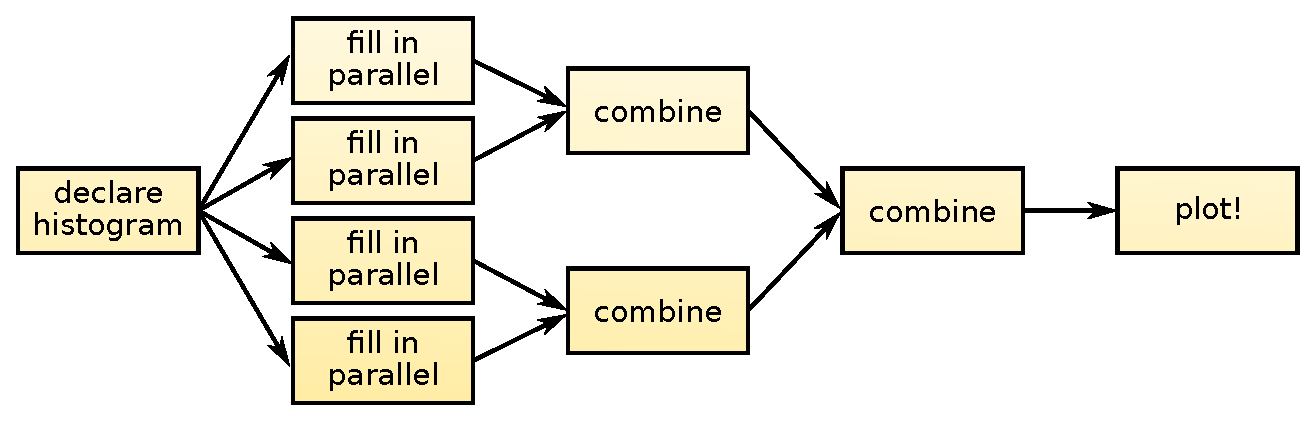
\includegraphics[width=\linewidth]{parallelization.pdf}

\vspace{-1 cm}
\[ \underbrace{\mbox{\hspace{2 cm}}}_{\mbox{head node}} \hspace{0.6 cm} \underbrace{\mbox{\hspace{8.125 cm}}}_{\mbox{executor nodes}} \hspace{0.625 cm} \underbrace{\mbox{\hspace{2 cm}}}_{\mbox{head node}} \]

\end{frame}

\begin{frame}{Designed for distributed workflows}
\vspace{0.5 cm}
\begin{block}{Parallel histogramming on a GPU}
\end{block}

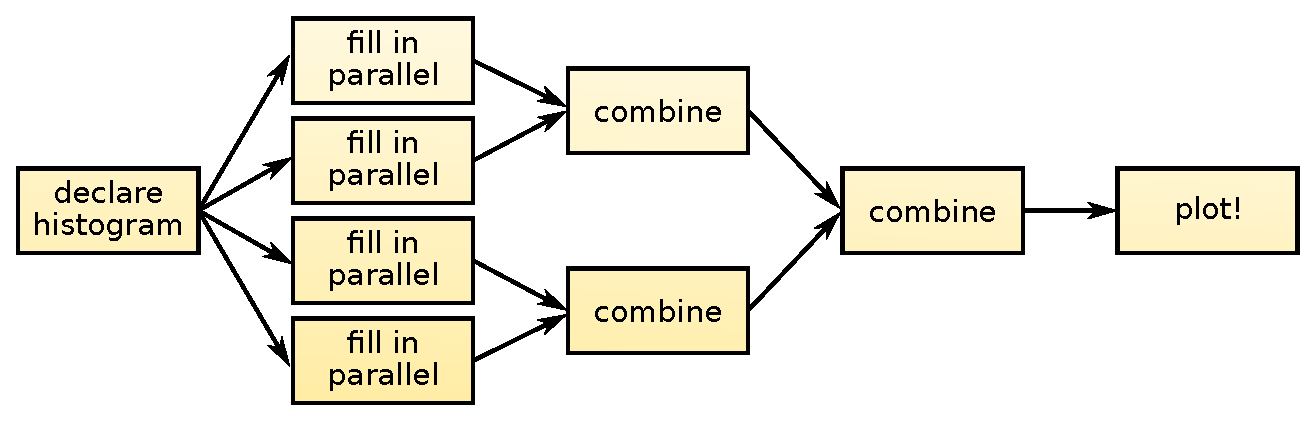
\includegraphics[width=\linewidth]{parallelization.pdf}

\vspace{-1 cm}
\[ \underbrace{\mbox{\hspace{2 cm}}}_{\mbox{host}} \hspace{0.6 cm} \underbrace{\mbox{\hspace{8.125 cm}}}_{\mbox{device}} \hspace{0.625 cm} \underbrace{\mbox{\hspace{2 cm}}}_{\mbox{host}} \]

\end{frame}

\begin{frame}{}
\hspace{-1 cm}\mbox{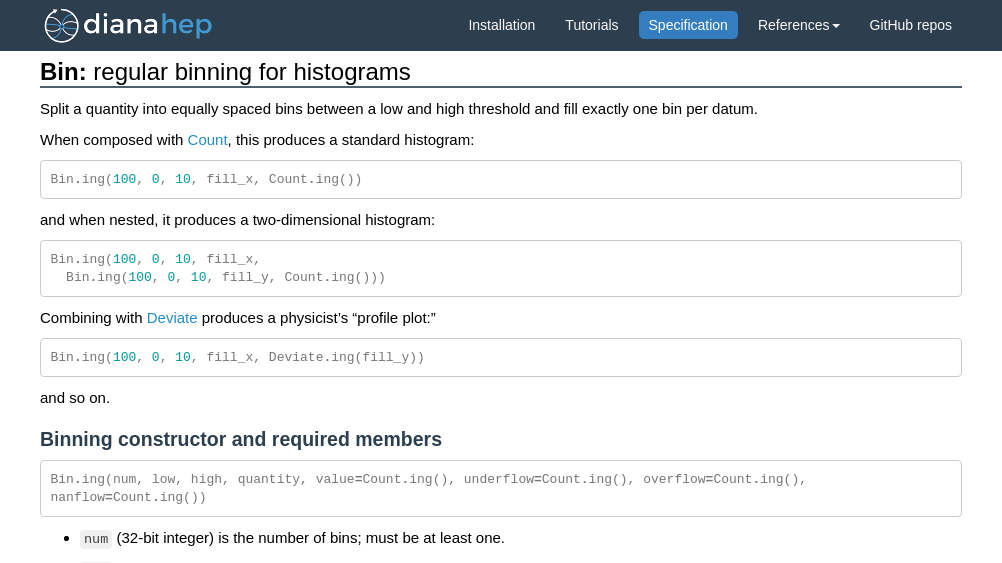
\includegraphics[width=16 cm]{spec1.png}\hspace{-5 cm}}

\vspace{-6.7 cm}
\hfill \fcolorbox{darkblue}{white}{\begin{minipage}{0.55\linewidth}
\vspace{0.75 cm}
\centering \textcolor{darkblue}{Screenshots from the specification}

\centering \textcolor{darkblue}{\url{http://histogrammar.org/docs/specification}}
\vspace{0.75 cm}
\end{minipage}} \hspace{-1 cm}
\vspace{6.7 cm}
\end{frame}

\begin{frame}{}
\hspace{-1 cm}\mbox{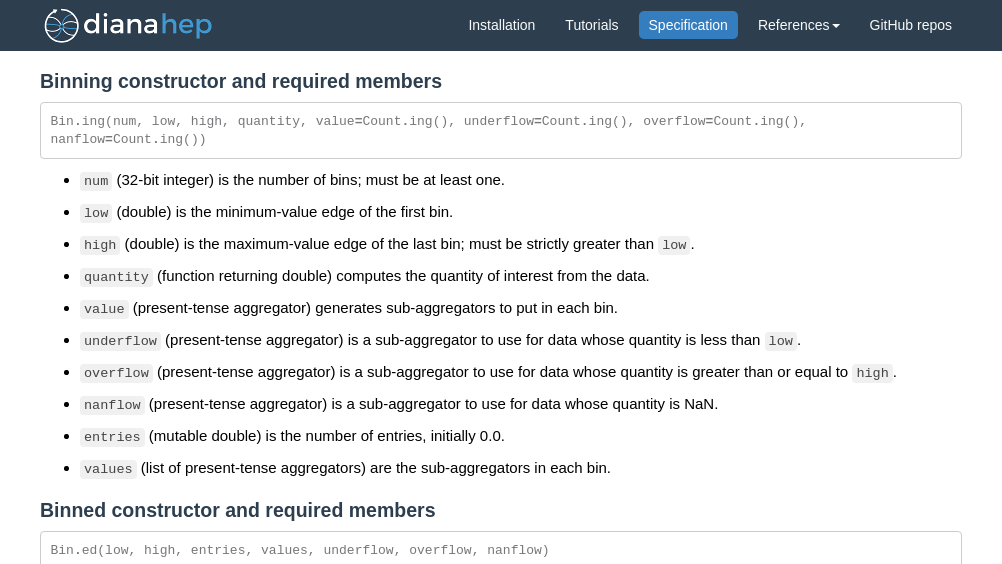
\includegraphics[width=16 cm]{spec2.png}\hspace{-5 cm}}
\end{frame}

\begin{frame}{}
\hspace{-1 cm}\mbox{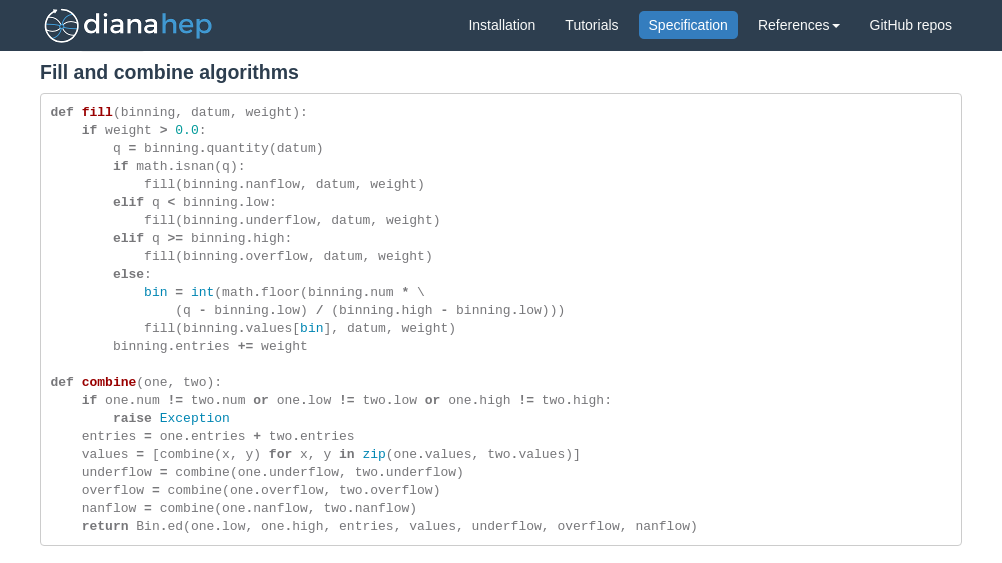
\includegraphics[width=16 cm]{spec3.png}\hspace{-5 cm}}
\end{frame}

\begin{frame}{}
\hspace{-1 cm}\mbox{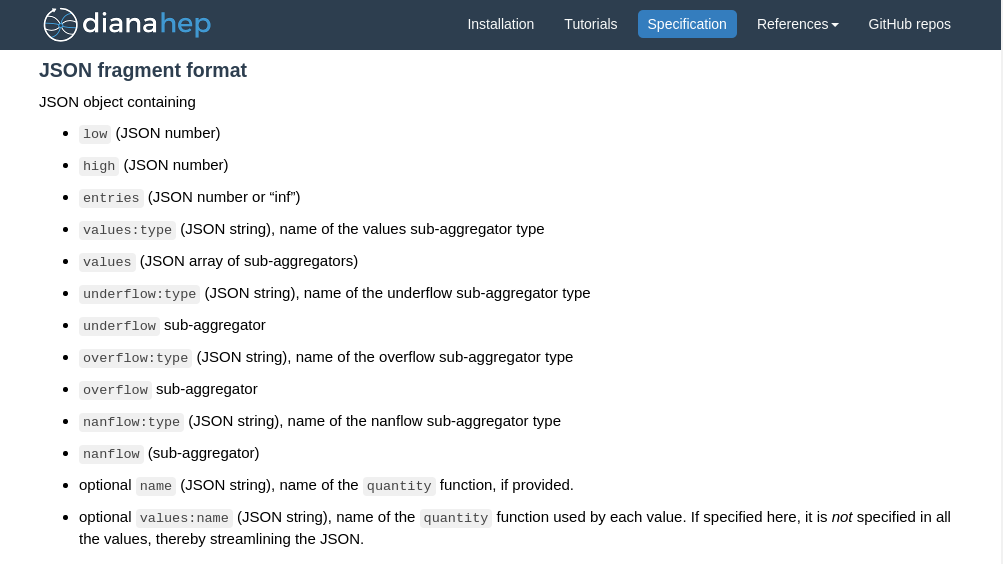
\includegraphics[width=16 cm]{spec4.png}\hspace{-5 cm}}
\end{frame}

\begin{frame}{}
\hspace{-1 cm}\mbox{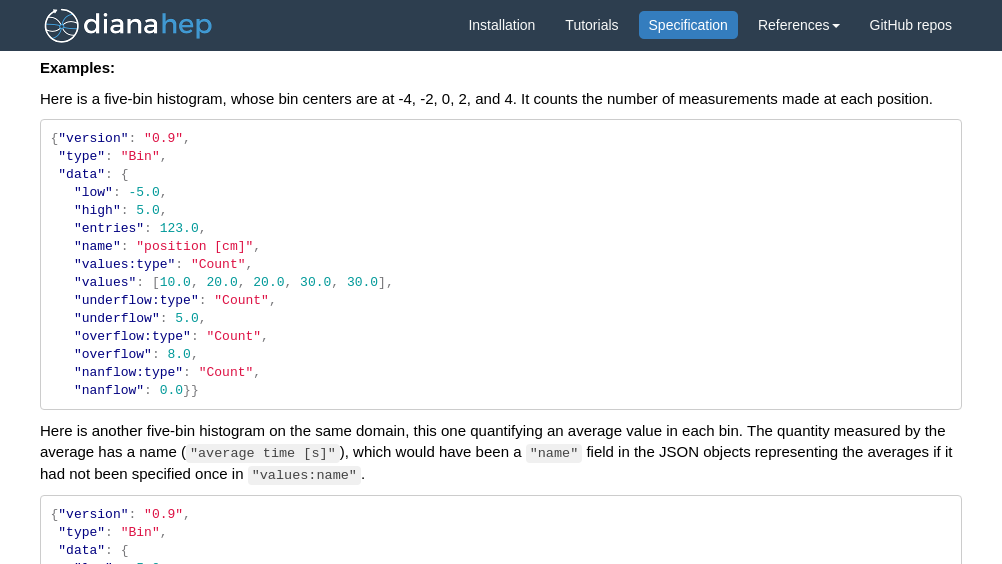
\includegraphics[width=16 cm]{spec5.png}\hspace{-5 cm}}
\end{frame}

\begin{frame}{}
\hspace{-1 cm}\mbox{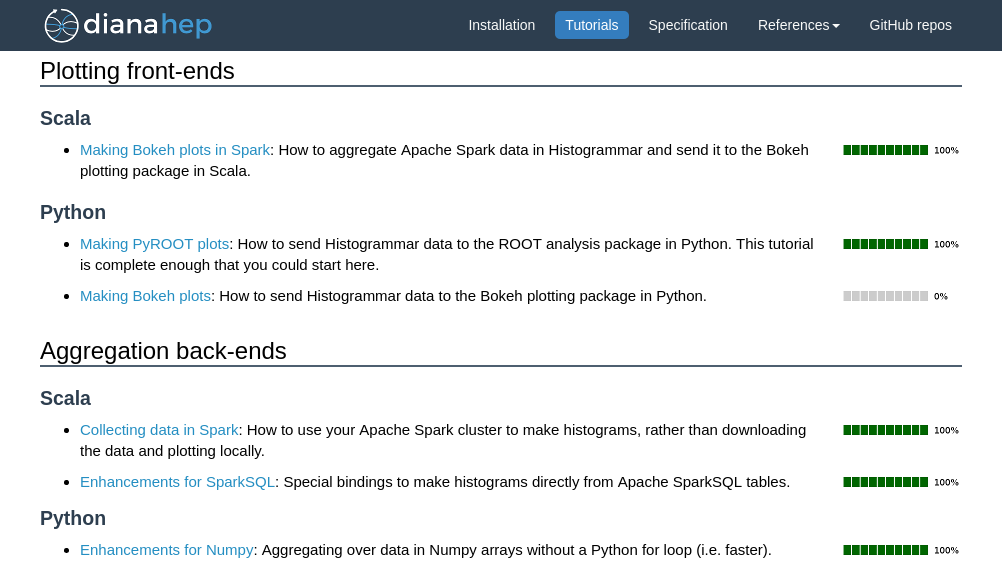
\includegraphics[width=16 cm]{tutorials.png}\hspace{-5 cm}}

\vspace{-7.5 cm}
\hfill \fcolorbox{darkblue}{white}{\begin{minipage}{0.65\linewidth}
\vspace{0.75 cm}
\centering \textcolor{darkblue}{Tutorials page}

\centering \textcolor{darkblue}{\url{http://histogrammar.org/docs/tutorials}}
\vspace{0.75 cm}
\end{minipage}} \hspace{-1 cm}
\vspace{7.5 cm}
\end{frame}

\begin{frame}[fragile]{Spark RDD and DataFrame back-ends}
\vspace{0.25 cm}
\textcolor{darkblue}{\large Spark RDD: provide an opaque function}

\begin{lstlisting}[basicstyle=\ttfamily\scriptsize\color{gray}]
implicit class DoublePow(x: Double) {
  def **(power: Double) = Math.pow(x, power)
}
\end{lstlisting}

\vspace{-0.25 cm}
\small
\begin{minted}{scala}
import org.dianahep.histogrammar._
val h = rdd.aggregate(
  Bin(10, 0, 100, {mu: Muon => Math.sqrt(mu.px**2 + mu.py**2)}))
  (new Increment, new Combine)
\end{minted}

\textcolor{gray}{(Statically typed to function arguments, hidden by type inference.)}

\vspace{0.1 cm}
\noindent\makebox[\linewidth]{\rule{\paperwidth}{0.4pt}}

\vspace{0.25 cm}
\textcolor{darkblue}{\large SparkSQL: provide a transformation on columns}

\begin{lstlisting}[basicstyle=\ttfamily\scriptsize\color{gray}]
implicit class ColumnPow(x: org.apache.spark.sql.Column) {
  def **(power: Double) = org.apache.spark.sql.functions.pow(x, power)
}
\end{lstlisting}

\vspace{-0.25 cm}
\small
\begin{minted}{scala}
import org.dianahep.histogrammar.sparksql._
val h = df.histogrammar(Bin(10, 0, 100, sqrt($"px"**2 + $"py"**2)))
\end{minted}
\end{frame}

\begin{frame}[fragile]{Python and Numpy back-end}
\vspace{0.35 cm}
\textcolor{darkblue}{\large Python: provide a lambda or a quoted expression}

\small
\begin{minted}{python}
from math import sqrt
from histogrammar import *
h = Bin(10, 0, 100, lambda muon: sqrt(muon.px**2 + muon.py**2))
h = Bin(10, 0, 100, "sqrt(px**2 + py**2)")
for mu in muons:
    h.fill(mu)
\end{minted}

\vspace{-0.35 cm}
\noindent\makebox[\linewidth]{\rule{\paperwidth}{0.4pt}}

\vspace{0.15 cm}
\textcolor{darkblue}{\large Numpy: provide a lambda or a quoted expression}

\small
\begin{minted}{python}
from numpy import sqrt
h = Bin(10, 0, 100, lambda muons:
                         sqrt(muons["px"]**2 + muons["py"]**2))
h = Bin(10, 0, 100, "np.sqrt(px**2 + py**2)")
h.fill.numpy(muons)
\end{minted}

\vspace{0.25 cm}
\uncover<2->{\fcolorbox{darkblue}{white}{\textcolor{darkblue}{Speedups range from nothing (string handling) to 100 times (depending on specific case).}}}
\vspace{0.25 cm}
\end{frame}

\begin{frame}[fragile]{JIT compilation}
\begin{minted}{python}
h = Bin(10, 0, 100, "sqrt(px*px + py*py)")   # C code
h.fill.root(muons)
\end{minted}

\begin{enumerate}\setlength{\itemsep}{0.3 cm}
\item Walk tree of aggregators to generate (cache-aware) C code instead of filling.
\item Compile the C code (in ROOT with LLVM).
\item Evaluate on a large dataset (in ROOT).
\item Update the original aggregator.
\end{enumerate}

\vspace{0.25 cm}
\uncover<2->{\fcolorbox{darkblue}{white}{\textcolor{darkblue}{Consistently 100 times faster than Python (and 30\% faster than generic C++ code).}}}
\end{frame}

\begin{frame}[fragile]{GPU code generation}
\vspace{0.5 cm}
\textcolor{darkblue}{\large Special case of JIT: generates parallel CUDA code.}

\begin{center}
\begin{minipage}{0.7\linewidth}
\small
\begin{minted}{python}
h = Bin(10, 0, 100, "sqrt(px*px + py*py)")
                        # expression in C

print h.cuda()          # prints CUDA code

h.fill.pycuda(muons)    # evaluates with PyCUDA
\end{minted}
\end{minipage}
\end{center}

\large
\begin{itemize}
\item<2-> Not intended as an accelerator (due to cost of sending data to GPU).
\item<3-> Intended as a convenience for developing GPU algorithms: the generated kernels are meant to be incorporated into other GPU projects so that those developers can see what they're doing.
\item<4-> Data reduction (even a simple counter) is tricky on a GPU. Histogrammar generates a function that outputs JSON, to be plotted externally.
\end{itemize}
\end{frame}

\begin{frame}{The unreasonable effectiveness of mathematics}
\vspace{0.5 cm}
\large
I learned (along the way) that all aggregators must be:

\vspace{0.25 cm}
\begin{uncoverenv}<2->
\hspace{1 cm}{\bf Additive}

\vspace{0.1 cm}
\hspace{1.5 cm}Independent of {\it whether} datasets are partitioned.

\vspace{-0.25 cm}
\[ \textcolor{darkblue}{\mbox{fill}(\mbox{data}_1 + \mbox{data}_2)} = \textcolor{darkblue}{\mbox{fill}(\mbox{data}_1) + \mbox{fill}(\mbox{data}_2)} = \textcolor{darkblue}{h_1 + h_2} \]
\end{uncoverenv}

\vspace{-0.2 cm}
\begin{uncoverenv}<3->
\hspace{1 cm}{\bf Associative}

\vspace{0.1 cm}
\hspace{1.5 cm}Independent of {\it where} datasets get partitioned.

\vspace{-0.25 cm}
\[ \textcolor{darkblue}{(h_1 + h_2) + h_3} = \textcolor{darkblue}{h_1 + (h_2 + h_3)} \]
\end{uncoverenv}

\vspace{-0.2 cm}
\begin{uncoverenv}<4->
\hspace{1 cm}{\bf Commutative}

\vspace{0.1 cm}
\hspace{1.5 cm}Independent of {\it order} of combining parts. \textcolor{gray}{\normalsize (Not essential, but convenient.)}

\vspace{-0.25 cm}
\[ \textcolor{darkblue}{h_1 + h_2} = \textcolor{darkblue}{h_2 + h_1} \]
\end{uncoverenv}
\end{frame}

\begin{frame}{The unreasonable effectiveness of mathematics}
\large
\begin{columns}
\column{0.5\linewidth}
\begin{center}
\bf \underline{RIP: AdaptivelyBin}
\end{center}

\begin{description}
\item[Want:] aggregator that determines binning from data.

\item[Tried:] each new datapoint is a new bin; merge closest bins.

\vspace{0.25 cm}
\begin{minipage}{\linewidth}
\scriptsize Ben-Haim and Tom-Tov, \href{http://www.jmlr.org/papers/volume11/ben-haim10a/ben-haim10a.pdf}{\textcolor{blue}{``A streaming parallel decision tree algorithm''}} {\it J. Machine Learning Research 11 (2010).}
\end{minipage}

\item[Problem:] result of {\ttfamily\small\textbf{fill}} depends on history of data seen; not additive or associative.
\end{description}

\begin{center}
\textcolor{darkblue}{Any ideas?}
\end{center}

\column{0.5\linewidth}
\begin{uncoverenv}<2->
\begin{center}
\bf \underline{RIP: Quantile}
\end{center}

\begin{description}
\item[Want:] approximate median or other quantiles.

\item[Tried:] incrementally minimize mean absolute error from target quantile.

\item[Problem:] result of {\ttfamily\small\textbf{fill}} depends on history of data seen; not additive or associative.

\mbox{ }
\end{description}

\begin{center}
\textcolor{darkblue}{Any ideas?}
\end{center}
\end{uncoverenv}
\end{columns}
\end{frame}

\begin{frame}{Want to get involved?}
\begin{center}
\begin{minipage}{0.55\linewidth}
\Large
\textcolor{blue}{\textbf{\url{http://histogrammar.org}}}

\begin{itemize}
\item Tutorials
\item Specification
\item GitHub organization
\item Maven Central/PyPI installation
\item Scaladocs/Sphinx reference
\end{itemize}
\end{minipage}
\end{center}
\end{frame}

\begin{frame}{Want to get involved?}
\begin{center}
\begin{minipage}{0.9\linewidth}
\Large
\textcolor{darkblue}{Want to\ldots}
\begin{itemize}\setlength{\itemsep}{0.35 cm}
\item wrap Histogrammar-Scala as HIVE UDAFs?
\item implement cache-aware JIT on the JVM?
\item design a modern C++ implementation ``the right way?''
\item integrate Histogrammar into R's data.frames or ggplot2?
\item develop a Javascript d3 front-end, thereby connecting Spark or GPUs to the web?
\end{itemize}
\end{minipage}
\end{center}
\end{frame}

\begin{frame}{Want to get involved?}
\vspace{0.5 cm}
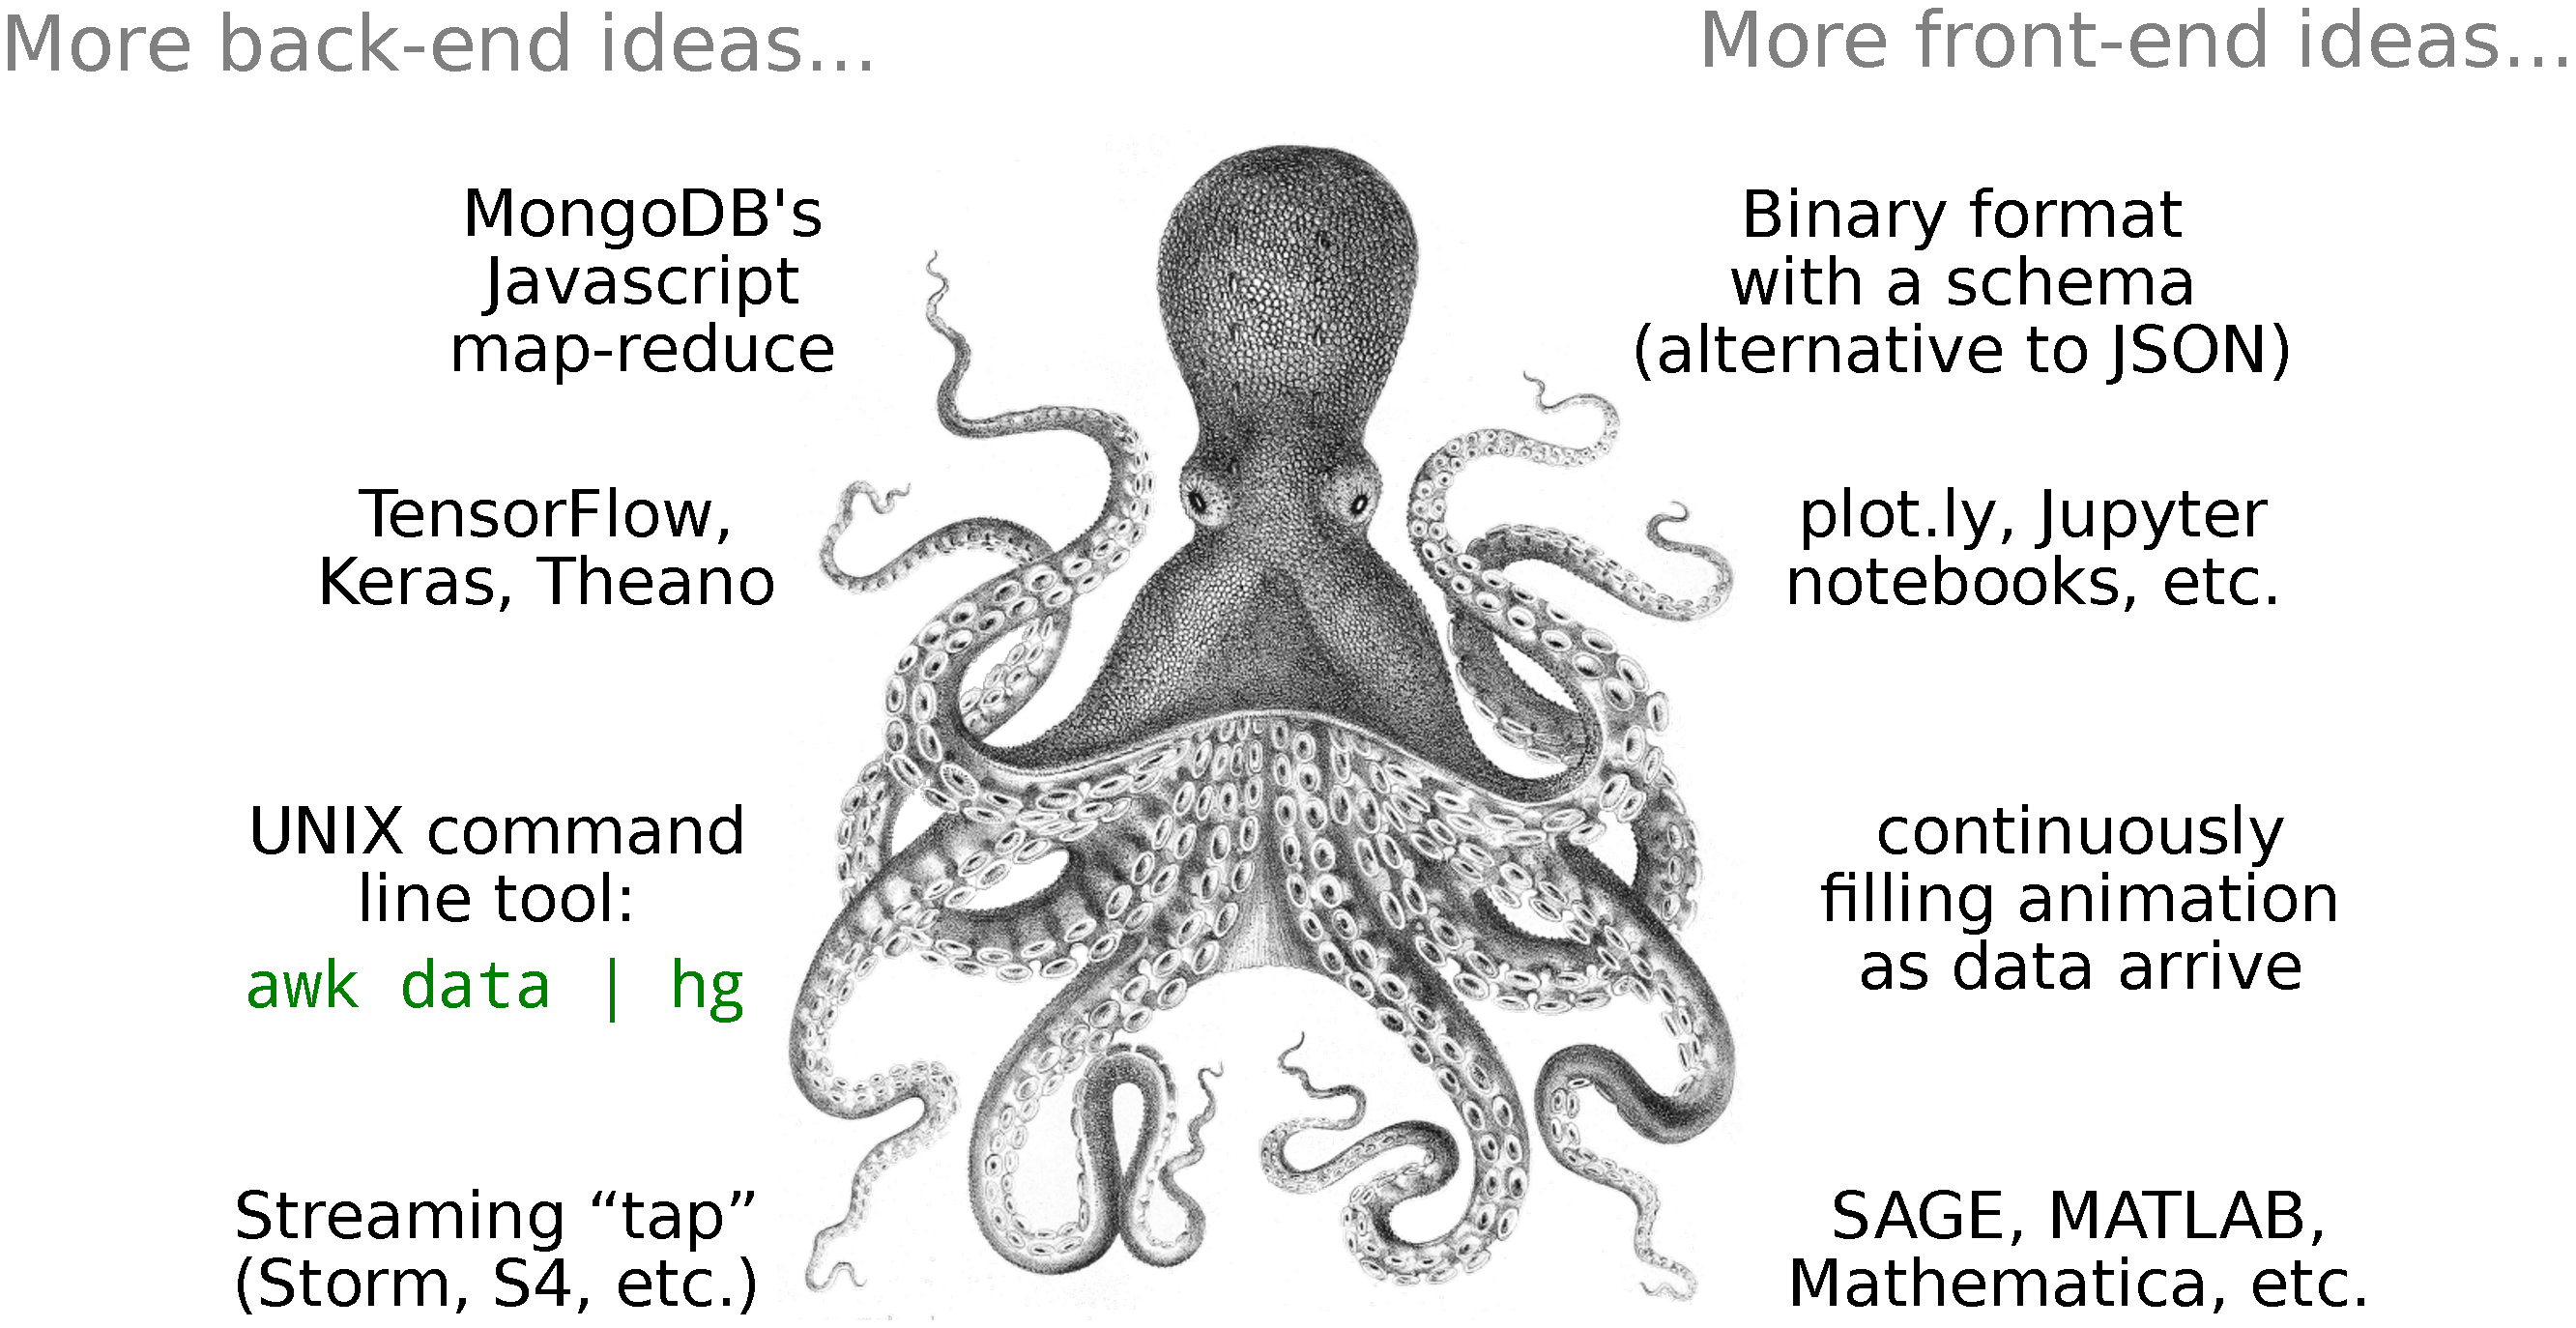
\includegraphics[width=\linewidth]{octopus_ending.pdf}
\end{frame}

\end{document}
